\section{中國大陸誤解香港帶來什麼後果?}

誤解往往帶來矛盾和對立。但在討論負面後果前,先說一些常常被忽略的,來自誤解的「正面後果」。

九七前後中國大陸對香港的官方宣傳大體上都是正面的,畢竟其目的就是要把主權移交書寫成一件民族復興的大喜事。有趣的是在九七後的十數年間,不少大陸傳媒利用了香港在中國大陸的正面公眾形象,和官方容許「唱好香港」的主調,借用香港新聞來批評中國大陸特別是官方的各種流弊。換言之,一百年前康有為和孫中山的做法,九七後再次在大陸傳媒中上演。

這兒舉三個例子。第一個例子來自二零一一年,時任民政事務局局長的曾德成在立法會回覆議員的提問時,報告了香港政府每年舉辦酒會或宴會的開支。到了第二天,香港本地報章對此事的關注十分有限,一般短短不足二百五十字便說完。然而這條在香港毫不起眼的新聞,在中國大陸卻引發熱議,各地媒體分別以數千字的專題文章介紹。曾德成的回應本身十分簡短,但這些文章談的不僅是這次立法會對答,而是把香港整套日常公共開支的監管制度整理出來,範圍也不限於原立法會提問所及的大型宴會,連一般宴請、以至公務車輛和公務外訪開支也論及。說到這兒,這些大陸媒體報道的用意已十分明顯:他們的題目不是香港,而是中國大陸的「三公經費」,也就是公費旅遊、公車消費和公款吃喝的問題,要借用香港的廉潔來諷刺中國大陸的腐敗。

這些報道對香港政府的各種制度,可以說是用祟拜的角度來書寫。例如說到時任行政長官曾蔭權的外訪經費時,就特別提到他曾經在休假時自己出錢買機票去美國,剛好遇上香港駐三藩市辦事處的活動,便順道担當主禮嘉賓,然而機票開支卻沒有報銷。來到今天,曾蔭權卻因涉貪案而纏上官司,回看這些歌訟式的報道也未免有點尷尬。

有些報道在刊登的時候已經明顯和香港本地的輿論不符,而且效果相當奇特。在二零一二年就有一宗大陸媒體和香港媒體立場倒轉的新聞。當時大陸媒體紛紛以「香港老太太迫停七百億元大橋」為題,大事報道香港一名六十多歲的居民通過向高等法院申請司法覆核,推翻了港珠澳大橋的環境評估。在許多中國大陸的評論當中,這位老太太就像是一名人民英雄一樣,而這次判決一方面代表了香港一般市民擁有極高的法治意識,同時也顯示出法院的大公無私以及政府對法治精神的尊重。有些評論更進一步從側面批評中國大陸「崇拜GDP,迷戀形象工程、面子工程」,進而指出尊重公民的訴求才是避免「群體性事件」的治本之道。

這些評論把香港說得這麼美好,實情又如何呢?因為大橋被迫停工,當時估計工程費用會增加六十五億(後來工程因為不相關的技術原因延誤及超支)。香港本地的親中報章拿著這點大書特書,聲稱訴訟延誤了香港的發展機遇,還指控老太太是受民主派政黨教唆才會出面訴訟,實際操作與她無關。老太太自己則因為受不了輿論壓力,多次表示後悔挑起了這場官司。這一系列的後續發展,和大陸傳媒所述的公民維權相距甚遠。

第三個例子來自二零一二年五月,《南方都市報》刊登的一篇專文,內容介紹香港各大專院校學生會的運作。文章一起始以香港學生到中國大陸交流為引子,提到學生會有能力把校長拉下台,把大陸同學嚇了一跳。這段引言所指的,是二千年港大校長鄭耀宗因為容許政治干預學術而被迫辭職的事件,專文也毫不含糊地介紹了這事件的來龍去脈。文章之後再介紹各學生會的校園抗爭歷史,並從制度上解釋為什麼它們有這些能力,從獨立注冊、獨立資金,到評議會和公投制度都解釋一遍。文章更把這些學生會的做事作方式引伸到香港社會對廉潔的追求,並指出香港很多著名的企業老板、議員和學者都出身於各大學的學生會。文章到今天仍在網上流傳,衝擊了不少大陸學生的思維,有學生幹部看罷文章後留言說,「感覺自己這個學生幹部白當了」。

跟上面兩個例子一樣,這篇專文對香港各大專院校的學生會的描述也未免過於美化。例如各學生會選舉的投票率其實十分低,選出來的不一定能代表同學的聲音,很多時候都會聽到批評學生會過於理想化、過於激進或沒有水平的聲音。然而從目的出發的話,上述三個例子所存的偏差都不重要,因為這些報道雖然說了很多關於香港的事情,主題卻不是香港,而是中國大陸,是大陸傳媒要借香港來指出大陸的問題。

上述借香港來批評中國大陸的報道手法近年來已不常見,大陸整體的言論監控相信是其中一個原因。以刊登學生會專文的《南方都市報》為例,所屬的「南方報系」本來就被認為屬自由派,而近年來所受的政治打壓似乎是越來越嚴重。但在這大背景下,特別針對香港的話語調整也十分明顯。

有調查發現二零一三年前後大陸媒體報道香港時所用的字詞明顯改變,之前以正面字詞比較常見,如「成功」、「第一」和「吸引」等,之後卻明顯地變得負面,如「激進」、「嚴重」和「矛盾」等。這轉變固然有客觀的背景,畢竟中港矛盾正是在這幾年間變得熾熱。梁振英於二零一二年上任香港特首後推行挑動敵我矛盾的管治政治,更使中港關係急轉直下。以港獨議題為例,在香港本來並不是一個公眾熱切討論的話題,卻被梁振英刻意挑起評擊,反而增加了社會的關注。相關的消息傳到中國大陸,也就形成香港負面新聞日益增加的基礎。

\begin{figure}[htbp]
    \centering
    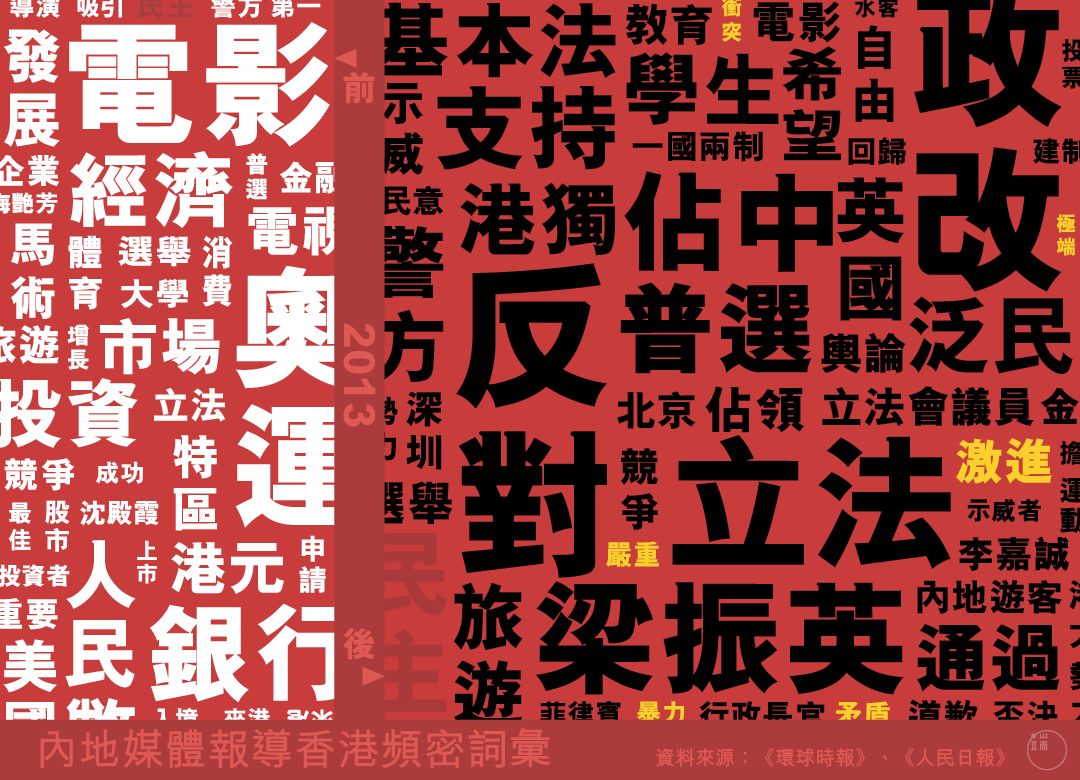
\includegraphics[width=0.7\textwidth]{c03/init-wordcloud.png}
    \caption{端傳媒:官方媒體從1997至2015年間有關香港報導的標題} 
\end{figure}

與此同時,有評論認為中國大陸的言論監控部門是樂意見到甚至鼓勵大陸媒體對香港的報道趨向負面。最起碼,先前所述「借港諷中」的報道手法,在這個新的言論環境中就難以發揮影響。批評香港人的抗爭行為,更可側面為中國大陸的維穩宣傳助威。這些對香港的負面新聞好像是一劑預防針一樣,事先在大陸民眾心目中貶低香港人的形象。如是者,日後即使香港人的政治訴求如何激烈,也不會得到大陸民眾的同情,並不會引發他們學習模仿。換句話說,「借港維穩」取代了「借港諷中」成為了報道香港新聞的新模式。例如上文提到的港珠澳大橋爭議,近年大陸傳媒就興起對此跟進報道時,但內容變成批判老太太濫用司法程序,大談香港法治制度不值得學習。

報道港聞的新模式在二零一四年的「反佔中」宣傳中走到巔峰。佔領中環是香港民主運動當中少有事先張揚的大型抗爭行動,而到了二零一四年年中,多數人已預期此行動將會發生。這時候,大陸媒體出現了大量「反佔中」專題,以極為負面的角度報道,卻對行動背後的訴求不作解釋。這些負面報道的目的當然不是要向中國大陸的民眾介紹香港面對的政治困局,而是要借機會責難「群體性事件」的「禍害」。佔領中環成為中國大陸維穩宣傳借題發揮的藉口,例如用來告誡民眾警剔外國勢力意圖在中國發動「顏色革命」製造社會混亂,儘管實際上並無證據顯示是次運動由任何外國勢力所促成或支持。

\begin{figure}[htbp]
    \centering
    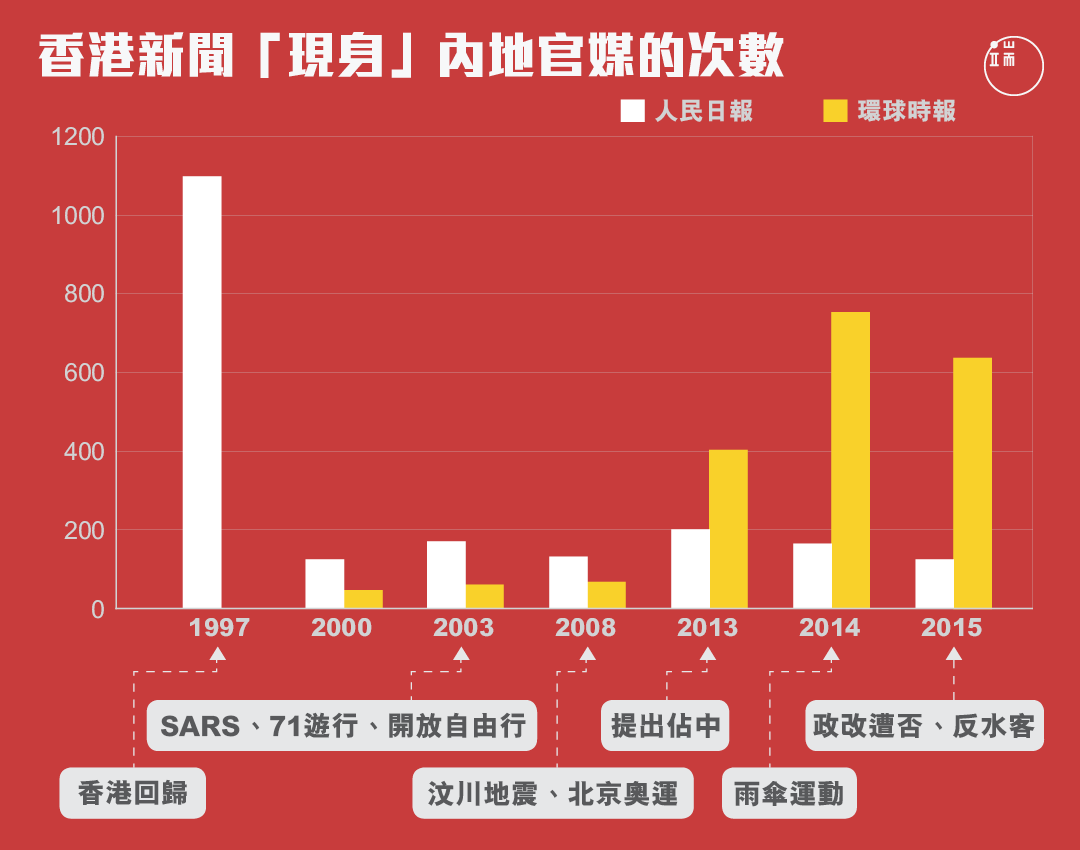
\includegraphics[width=0.7\textwidth]{c03/init-h-kappearance.png}
    \caption{端傳媒:《環球時報》設定了內地媒體關於香港形象的新議程} 
\end{figure}

港獨議題的出現,更成為中國大陸維穩宣傳一個「大顯身手」的機會。愛國主義教育是中共自八九民運後刻意經營維護政權的重要工具,港獨議題的迅速冒升很大程度上是因為它可輕易被愛國主義吸納成為宣傳演練的題目。在此脈絡下,香港人的民主訴求只要被套上港獨的帽子,就會立即失去正當性,這些民主訴求就不會蔓延到中國大陸。港獨本身是否事實並非要旨,重要的是這個題目可以被愛國主義教育所挪用,所以很多本來和港獨不相關的人和事都可以忽然變成港獨漫延的證據。例如二零一六年年末有市民發起穿著二次大戰時期英聯邦守軍的軍服在鬧市穿梭,紀念當年為港捐軀的士兵,這活動的圖片卻被大陸媒體扭曲為「港獨份子建軍招搖過市」,儘管活動組織者強調他們和港獨毫無關係。這樣的假新聞在香港當然只會被視為笑話,但在中國大陸卻被廣泛轉載,引發不少大陸民眾義憤難平。

\begin{figure}[htbp]
    \centering
    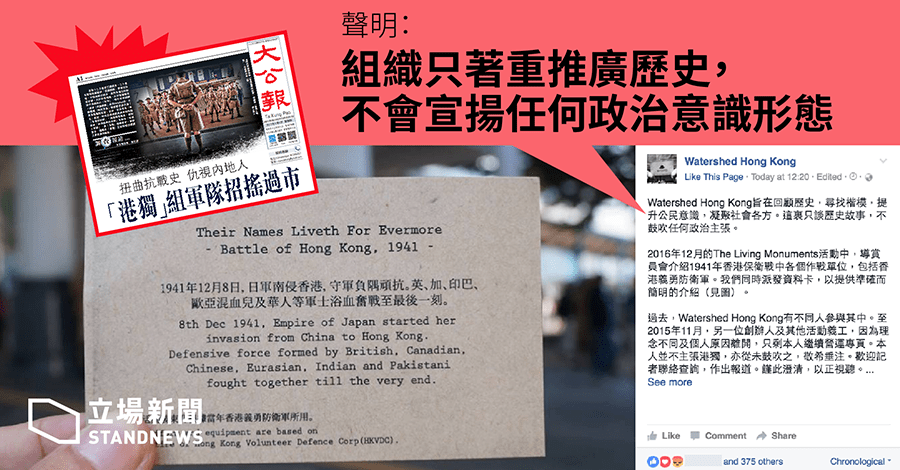
\includegraphics[width=0.7\textwidth]{c03/sn-battleof-hk.png}
    \caption{立場新聞:團體澄清只著重推廣歷史} 
\end{figure}

拉闊一點來看,「香港」二字按中國大陸的政治需要成為被隨意挪用的符號,引發出各式各樣和香港本身不一定相乎甚至相關的解讀,並不是一件新鮮的事情,甚至可以說是香港自開埠以來就要面對的現實。要指出這些挪用的不足,也不是要說這些解讀毫無價值。英殖香港成為晚清改良派和革命黨人的宣傳工具,也可理解為一件對當時的中國有益的事情。不過,近年中國大陸對內政治空間急速收縮,對外政治想像大幅改變,而中港關係又走向越來越密切的時候,偏見就可以帶來嚴重惡果。

書寫和故事本身的互動關係,常常會以瞎子摸象為比喻。閉上雙眼觸摸一只大象,摸到尾的以為是繩,摸到頭的以為是石,這本來正常不過,也不至於要譴責當中任何一人的誤解。但如果有人堅持己見,批評其他人的所得到是邪說,還禁止別人用其他的方式來認識,就會無法知道大象的存在,最終可能死在象蹄之下。

近年來,中國大陸有關香港的宣傳,要不是把所有中央對港政策都解讀為「獻禮」或「讓利」,就是直接批評香港的政治局勢和市民的政治訴求。加上大陸言論控制信息不通,各種不實信息得以流傳,如誤稱九七年金融風暴港府的金融市場保衛戰是由中央政府出資。另一個經典案例,是大陸傳媒常把廣東省東江供水香港視為中央政府對香港的支持,其實深圳和東莞同樣要靠東江供水,但對香港收取的水價卻是深圳和東莞的五倍。二零零九年廣東出現旱災,香港政府曾提議減少供水以舒緩廣東旱情,卻被廣東省方面拒絕,足以說明廣東省視供水為商業交易,談不上刻意讓利。

由於中港關係的實際情況往往不能在大陸媒體審查下得到全面報道,類似上述對中港關係的錯誤認識在中國大陸可謂層出不窮,從食物、能源、投資到其他經濟領域數之不盡。不少大陸民眾基於這些錯誤觀念對香港出現「要不是中央照顧,香港早就完蛋了」的「恩主心態」,覺得香港是「被寵壞了的孩子」。而當他們帶著這種心理來到香港社會和香港人交往,自然產生巨大落差,矛盾被進一步激發。

民間社會的認識落差可怕,但政府的認識落差恐怕更叫人擔憂。中國法律學者強世功曾在中央人民政府駐香港特別行政區聯絡辦公室(中聯辦)做研究工作,後來出版《中國香港:文化與政治的視野》一書,講述他研究出來的香港近代史,被視為中國官方香港論述的理論依據。不過,此書內容卻被文化界的陳冠中批評為牽強武斷,而且充滿內部矛盾。如果中國政府本身都是基於不準確的認識和理解下制訂其對港政策,其決定必然會在香港製造反彈,中港矛盾越演越烈也是正常不過的結果。

與此同時,這些官方針對香港的反宣傳其實對中國大陸的老百姓來說也有壞處,背後的問題和反日或反美示威相當類似。當各式各樣的反對活動都被官方禁止,就只有「愛國無罪」,各種問題就很容易被簡化為是出於「外國敵對勢力」的打擊,自身的問題和責任就被輕輕帶過,既得利益者就可以躲在愛國主義的旗幟下進一步套取各種好處。

最後,得說明在認識落差這回事上面,香港人自己也好不到那裡。香港人對中國的認識同樣是充滿偏見的,香港人對香港自身的理解和認同也是建基於許許多多迷思,而它們也同樣反過來限制香港的發展。不過如同前文的討論,僅僅譴責這些誤解並不足夠,更重要的是去問為什麼這些誤解會流行起來,而阻礙其他理解出現的原因又是什麼。

伸延閱讀:

強世功(2008):《中國香港:文化與政治的視野》,香港:牛津大學出版社。

陳冠中(2012):《中國天朝主義與香港》,香港:牛津大學出版社。

駱穎佳(2016):〈驚異的空間政治:後社會主義國族論述對香港的異托邦想像〉,《邊緣上的香港:國族論述中的(後)殖民想像》,香港:印象文字。